\documentclass{standalone}
\usepackage{standalone}

\begin{document}

\subsection{Extraction}
The region information we get from the previous step is used here to extract the plate image from the original image. We also rotate the image to match with the rotation angle found in previous step. This rotation is done by calculating a rotation matrix of scale $1$ using a OpenCV function:
\begin{lstlisting}[language=Python]
# Calculating rotation matrix M
M = cv2.getRotationMatrix2D(\
		     (center_y, center_x), rotation, 1.0)
\end{lstlisting}

The variable $rotation$ here is calculated from the $minAreaRect$'s $angle$ using Equation \ref{eq:ExtractionAngle}.
\begin{equation} \label{eq:ExtractionAngle}
rotation = 
\begin{cases} 
	-angle, & \mbox{if } angle \leq 45\\
    90 - angle, & \mbox{if } angle > 45
\end{cases}
\end{equation}

For convenience, the extracted plate image is rescaled into a dimension of $500 \times 250$. Figure \ref{fig:FinalPlate} shows a sample.
\begin{figure}
    \centering
    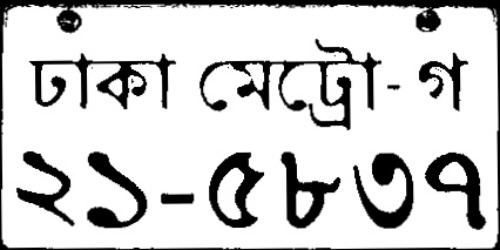
\includegraphics[width=.7\linewidth]{./img/sample/stage10.jpg}
    \caption{The extracted plate after rotation and scaling}
    \label{fig:FinalPlate}
\end{figure}



\end{document}